% Camera-ready revision of WiCOMM-2026 paper 167. Built on the submitted manuscript
% (archive/manuscripts_before_revision/paper.tex); tables are generated from raw runs by
% experiments/camera_ready_manuscript_data.py, figures by experiments/make_fig_*_cr.py.
\RequirePackage[T1]{fontenc}
\documentclass[conference,a4paper]{IEEEtran}
\IEEEoverridecommandlockouts

\usepackage{cite}
\usepackage{amsmath,amssymb}
\usepackage{graphicx}
\usepackage{booktabs}
\usepackage{url}
\usepackage[hidelinks]{hyperref}
\graphicspath{{figures/camera_ready/}}
\setlength{\textfloatsep}{7pt plus 2pt minus 2pt}
\setlength{\dbltextfloatsep}{7pt plus 2pt minus 2pt}

\newcommand{\GI}{G\textsubscript{1}}
\newcommand{\GII}{G\textsubscript{2}}
\newcommand{\GIII}{G\textsubscript{3}}
\newcommand{\GIV}{G\textsubscript{4}}

\begin{document}

\title{Fail-Closed or Fail-Degraded? A Simulation Study \\of Forced Assurance
Loss in Contested Multi-Hop QKD Networks}

\author{
\IEEEauthorblockN{Lakshya Jain}
\IEEEauthorblockA{\textit{Maharaja Agrasen Institute of Technology}\\
Delhi, India\\
10jainlakshya@gmail.com}
\and
\IEEEauthorblockN{Siddhi Arora}
\IEEEauthorblockA{\textit{Noida Institute of Engineering and Technology}\\
Greater Noida, India\\
Sid.arora1701@gmail.com}
}

\maketitle

\begin{abstract}
In multi-hop trusted-relay quantum key distribution (QKD), every hop of a relayed
path consumes secret key, so key is a per-link resource that can run out. What a
network should then do is still open: ITU-T Y.3803 allows falling back to a symmetric
cipher, while a recent layered design fails closed and treats the switch as a
downgrade attack. We measure the trade-off on an eight-node tactical relay formation
and four other graphs with minimum cuts of two to four links, against an adversary
that raises the quantum bit error rate until targeted links stop generating key. We
define \emph{forced assurance loss}, the fraction of requests entitled to an
information-theoretically secure (ITS) key that are served without one, and the
\emph{downgrade-forcing cost}, the attack effort needed to cause it. Holding the
formation's two-link cut for 24 hours, with stores at 2\% of usable capacity, drops
fail-closed service from 97.5\% to 6.7\%. Fail-degraded operation still serves
97.5\% of requests, but only 6.6\% at their authorised grade, and pushes 90.1\% of
entitled requests below an ITS key. Forcing needs a per-link capability, a
cost-weighted cut and endurance: with full stores the same attack forces nothing
within 24 hours. A learned grade controller tested on held-out seeds gains little
utility and raises below-ITS payload exposure. QKD resilience reports should
therefore state the assurance grade of the traffic served.
\end{abstract}

\begin{IEEEkeywords}
Quantum key distribution, trusted-relay networks, key management, post-quantum
cryptography, graceful degradation, military communications.
\end{IEEEkeywords}

\section{Introduction}
Consider a brigade in mountainous terrain whose link to the rear area is a chain of
relay sites carrying command circuits rekeyed every few minutes, imagery encrypted at
one-time-pad rates and bulk, delay-tolerant logistics. Suppose the network can no
longer supply quantum key for all of it. Refusing service gives the commander an
outage to act on. Keeping the circuit up and rekeying the imagery link with a
computationally secure algorithm shows nothing, and the loss surfaces only at audit.
Which failure is worse is unclear.

Trusted relays make the question pressing. Beyond one quantum channel's reach, keys
are forwarded hop by hop: each node re-encrypts the end-to-end key under its neighbour
key with a one-time pad and an ITS authenticator~\cite{salvail}. An $n$-hop path thus
consumes key on \emph{every} one of its $n$ links, and at free-space rates of order $10^{2}$\,bit/s per hop the binding constraint is the key supply.

Standards, key managers and layered designs treat exhaustion in opposite ways. Some
permit degradation: a symmetric cipher may replace missing one-time-pad key if the
method is recorded~\cite{itu3803}, deployments do so~\cite{makris}, and key managers
can put both branches under policy control~\cite{tysowski}. Others fail closed,
tearing down the tunnel to prevent a \emph{downgrade attack}~\cite{spooren}. The worry
is older than either mechanism: an adversary who cannot steal quantum keys may deny
them instead, precisely to \emph{force} classical cryptography into
use~\cite{schartner}.

To our knowledge neither option has been measured on a multi-hop network, and no study
has asked what each costs or what an adversary must spend to force the choice.
Refusal turns attack effort into a visible outage and degradation into a silent loss of assurance, so operators choose without data.

Our contributions are: (i) a threat-aware model in which stored key outlives
generation and three failure surfaces stay separate (\S\ref{sec:link}); (ii)
\emph{forced assurance loss} on traffic \emph{entitled} to ITS key, reported beside
floor-compliant service, the \emph{downgrade-forcing cost} with per-link attack costs,
and a cut condition predicting service under a held cut (\S\ref{sec:metrics}); (iii)
evidence on five graphs that forcing needs capability, a cut and endurance, with
routing and retargeting analyses (\S\ref{sec:head}--\S\ref{sec:sens}); (iv) an audit
of a learned grade controller on disjoint seeds (\S\ref{sec:audit}); and (v) a check of
the key accounting against published measurements (\S\ref{sec:valid}).

\section{Related Work}
\begin{table}[t]
\caption{Dimensions addressed by representative trusted-relay QKD studies, in the
order the text discusses them.}
\label{tab:pos}
\centering\footnotesize
\setlength{\tabcolsep}{3.5pt}
\begin{tabular}{@{}lccccccc@{}}
\toprule
Work & MH & KS & TC & AD & SW & FB & FA\\
\midrule
Routing~\cite{vanduijn,johann,hao} & \checkmark & \checkmark & & & & & \\
\addlinespace[2pt]
Mehic \emph{et al.}~\cite{mehic} & \checkmark & \checkmark & \checkmark & $\circ$ & & & \\
Cao \emph{et al.}~\cite{cao} & \checkmark & \checkmark & $\circ$ & & & & \\
\addlinespace[2pt]
Tysowski \emph{et al.}~\cite{tysowski} & \checkmark & \checkmark & \checkmark & & & \checkmark & \\
Sanz \emph{et al.}~\cite{sanz} & \checkmark & & \checkmark & & & \checkmark & \\
Zhu~\cite{zhu} & $\circ$ & \checkmark & \checkmark & & & \checkmark & $\circ$\\
Makris \emph{et al.}~\cite{makris} & \checkmark & $\circ$ & & $\circ$ & & \checkmark & \\
Spooren \emph{et al.}~\cite{spooren} & \checkmark & & & $\circ$ & & $\dagger$ & \\
\addlinespace[2pt]
Li \emph{et al.}~\cite{li} & \checkmark & \checkmark & & \checkmark & & & \\
Ghourab \emph{et al.}~\cite{ghorab} & \checkmark & \checkmark & & \checkmark & \checkmark & & \\
Hafeez \emph{et al.}~\cite{hafeez} & \checkmark & \checkmark & & \checkmark & \checkmark & \checkmark & \\
\bottomrule
\end{tabular}
\begin{flushleft}\footnotesize
\emph{MH} multi-hop; \emph{KS} scarcity binds; \emph{TC} traffic classes;
\emph{AD} adversary; \emph{SW} pressure swept; \emph{FB} computational fallback;
\emph{FA} assurance loss on entitled traffic. \checkmark~addressed; $\circ$~partial;
$\dagger$~specified, fails closed.
\end{flushleft}
\end{table}

Trusted-relay QKD research follows four largely separate lines. Routing work asks
which path a request should take when key is scarce~\cite{vanduijn,johann,hao,cvitic},
and quality-of-service work adds priority classes and admission control~\cite{mehic}
or couples key supply to an optical control plane~\cite{cao}. Both share one outcome
model: a request gets a path with key on every hop or is blocked. Priority therefore
decides \emph{which} requests receive quantum key, never \emph{what kind}.

The third line deals with exhaustion. Standards and key managers allow recorded
substitution~\cite{itu3803,tysowski}, deployments implement it~\cite{makris}, graded
delivery has been specified~\cite{sanz} and costed~\cite{zhu}, and a layered design
fails closed~\cite{spooren}. Single-link studies fall back to a KEM on attack or
failure~\cite{agalya,hernandez} but score it by availability, which counts a
post-quantum-only session as served. The fourth line adds an adversary (key-store
depletion by denial of service~\cite{mehicdos}, attack-radius minimisation~\cite{li},
zero-trust relays~\cite{ghorab}, swept degradation for 6G~\cite{hafeez}) but keeps the
served-or-blocked outcome, so the threat of forced classical
cryptography~\cite{schartner} is missing.

Table~\ref{tab:pos} covers studies that model key supply over more than one relay hop.
Its assurance column has no full mark: none of the studies we found reports the
fraction of \emph{entitled} traffic served below ITS, and the nearest,~\cite{zhu}, is
neither restricted to entitled traffic nor swept. We know of no prior work that
compares the two fail modes on a multi-hop network or prices what forcing the choice
costs an adversary.

\section{System Model}
Because \emph{hybrid} denotes a key combiner that is secure if one component
survives~\cite{ietfhybrid}, a QKD$\rightarrow$post-quantum substitution is not hybrid;
we call it a labelled grade downgrade.

\begin{figure}[t]
\centering
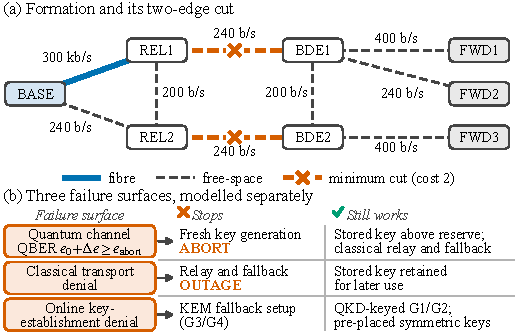
\includegraphics[width=\columnwidth]{fig1_architecture.pdf}
\caption{(a) The eight-node formation, per-link secret key rates and the minimum cut isolating its forward posts. (b) The three failure surfaces, which the model keeps
separate (\S\ref{sec:link}).}
\label{fig:arch}
\end{figure}

We model (T1) an eight-node formation (rear node, two relays, two brigade nodes, three
forward posts; one 300\,kbit/s fibre and eight 200--400\,bit/s free-space links,
Fig.~\ref{fig:arch}a) and (T2) a depth-$d$ chain with one longer alternate for
$d\ge2$. An eight-node ring, a $3\times3$ grid and 3- and 4-path parallel graphs, each
with one source, one sink and 240\,bit/s links, add minimum cuts of two, two, three
and four. Sessions run from the rear node to the forward posts and debit the reservoir
of every hop. Every formation session crosses one of two 240\,bit/s links, so the
fibre's surplus is stranded one hop from the bottleneck.

Reservoirs follow QKDNetSim's key-buffer semantics with its SECOQC example
values~\cite{qkdnetsim}: capacity $52\,428\,800$, threshold $11\,324\,620$ and a
protected reserve of $1\,048\,576$ bits, the role SECOQC gave to key held for
authentication~\cite{peev}. Overflow is discarded; we found no published capacity from
vendors or ETSI~\cite{etsi014}. Distilled key remains spendable after generation
stops, so an attack on the quantum channel cuts off replenishment but leaves the
stock. Stores start at a declared usable fill, 2\% (1.03\,Mbit per link) in the main
runs.

Sessions are served at four grades: \GI\ one-time pad (key $=$ payload bits); \GII\
QKD-keyed symmetric (256\,bit, ITS-\emph{delivered} key under a computational cipher);
\GIII\ hybrid QKD\,$\oplus$\,ML-KEM-768 (128\,bit plus KEM); \GIV\ ML-KEM-768 only.
Each class has an \emph{authorised floor}. If the floor cannot be met, the controller
either blocks at the deadline (\textsc{fail\_closed}) or serves below the floor at once
and records an auditable violation (\textsc{fail\_degraded}).

\subsection{Link model and adversary}\label{sec:link}
An adversary who raises the noise past the security threshold halts key
generation~\cite{alleaume}, so a fixed degraded rate is indefensible. A link
is \textsc{nominal} ($R_0$), \textsc{degraded} ($R_0\rho(e)$), in \textsc{abort} (no
fresh key, $e\ge e_{\mathrm{abort}}$) or in \textsc{outage} (no classical transport),
with
\begin{equation}\label{eq:rho}
\rho(e)=\left[\frac{\max\!\left(0,\,1-(1+f)H_2(e)\right)}
{1-(1+f)H_2(e_0)}\right]^{\gamma},
\end{equation}
$f=1.16$ and $e_0=0.03$~\cite{sasaki}. We report $\gamma=1$ (asymptotic BB84) and
$\gamma=3.4$, a steeper shape matched to one datapoint from another
modality~\cite{sasaki} for illustration only. The threshold $e_{\mathrm{abort}}=0.075$ is an engineering value (the NEC--NICT engine of~\cite{sasaki} codes only below 7.5\%), with
0.11 as a sensitivity.

QBER pressure stops generation but leaves the classical channel intact, so stored key
can still be relayed and any fallback still works. Classical-channel denial halts
post-processing and transport~\cite{mehic}, and denial of the online key-establishment
service blocks a KEM fallback but not QKD-keyed grades or pre-placed keys
(Fig.~\ref{fig:arch}b). Detector blinding~\cite{lydersen} raises no QBER and is
invisible here. The adversary injects excess QBER $\Delta e$ on the links it
buys~\cite{schartner}, at relative cost 1 per free-space link and 10 for the fibre (1
and 100 as sensitivities); these are scenario weights, not measured expenditure. It chooses targets by static betweenness per unit cost, by \emph{residual} betweenness
recomputed after each removal, by the cost-weighted minimum cut, or online from
committed routes.

\subsection{Key accounting and traffic}\label{sec:acct}
Relaying $K$ bits of key across one hop costs
\begin{equation}\label{eq:debit}
q=K+M_{\mathrm{meta}}+n_{\mathrm{auth}}\,t,
\end{equation}
with metadata $M_{\mathrm{meta}}=240$\,bit (Y.3803 relays a key file) and a tag
$t=127$\,bit~\cite{walenta} charged per authenticated message~\cite{fung}. No
specification fixes the count $n_{\mathrm{auth}}$ per delivery. Two is a lower bound
and field data imply about 7 (\S\ref{sec:valid}), so we use 7 unless stated (a \GII\
debit of 1385\,bit per hop), with 2 and 40 as sensitivities.

Demands follow measured deployments. C2: 2048\,bit, floor \GII, 5\,s deadline,
$\lambda=0.05$\,s$^{-1}$ (256\,bit/min per encryptor~\cite{stucki}). ISR:
144\,000\,bit, floor \GI, 30\,s, i.e.\ a 60\,s session of 2.4\,kbps one-time-pad
voice~\cite{chen}. LOG: 320\,000\,bit~\cite{chen}, floor \GIII, 120\,s,
$\lambda=0.03$\,s$^{-1}$. Priority follows this order. At 0.02\,s$^{-1}$ (ISR factor
1) the mean debit across the formation's cut would exceed six times its 480\,bit/s
supply, which no store could fund, so ISR runs at factor 0.1, or 0.002\,s$^{-1}$
(397\,bit/s in total across the cut, 83\% of supply). Factors 1 (overload) and 0.03
(light) are sensitivities.

\subsection{Metrics and a cut condition}\label{sec:metrics}
Of $N$ arriving requests, let $S$ be those served within their deadlines and $D\subseteq S$ those below their authorised floor:
\begin{equation}\label{eq:metrics}
A=|S|/N,\qquad Q=|S\setminus D|/N,\qquad L=|D|/N,
\end{equation}
so $A=Q+L$, splitting availability into compliant service $Q$ and below-floor service
$L$, which includes post-quantum-only fallback. \emph{Forced assurance loss}
$F=|D_{\mathrm{ITS}}|/|E|$ is the number of requests entitled to ITS key (floors \GI,
\GII) served at \GIII\ or \GIV, divided by all entitled arrivals including blocked
ones, so both modes share one denominator. An ISR request served at \GII\ misses its
floor (counted in $L$) but keeps an ITS-delivered key (not in $F$). Payload weighting
gives $F_B$, and class weights $(5,2,1)$ and $(10,3,1)$ for (C2, ISR, LOG) give a
second reweighting; both are exposure proxies.

For a cut $\delta(W)$ separating the rear node from the forward posts, with usable
stock $U_e(0)$ and generation $G_e(T)$ on cut link $e$, every compliant session
completed by $T$ debits at least its floor debit $q_s$ from some cut link:
\begin{equation}\label{eq:cut}
\textstyle\sum_{s\in\mathcal{C}_T} q_s\;\le\;\sum_{e\in\delta(W)}\bigl[U_e(0)+G_e(T)\bigr].
\end{equation}
Holding every cut link past abort sets $G_e=0$, so at demand $\bar D=\sum_c\lambda_cq_c$
compliant service lasts at most $T^\ast=\sum_eU_e(0)/\bar D$, or 1.44\,h for the
formation at 2\% fill. The condition is necessary but not sufficient: a test graph of
three two-hop branches strands 400 bits per branch and serves six requests where the
bound allows seven.

\section{Experimental Setup}\label{sec:setup}
We use discrete-event simulation at 1\,s resolution. Admission checks every hop before any debit, and a pending request retries until its deadline, within which \GIII/\GIV\ must also finish a 0.35\,s online setup. Arrivals and the attack last 24\,h, and pending requests are followed to their deadlines. A declared initial fill replaces
a warm-up, since full stores drain only under an overloaded ISR class. Free-space
generation and each link's transport fail independently (mean up 3600\,s, down
120\,s); a severe-weather variant (900/600\,s) runs independently or switches all
free-space generation together. Under \emph{common random numbers} every policy and
attack sees identical arrivals and environmental draws per seed, so attack effects are
paired differences against the unattacked run. We report means of per-seed fractions
with 95\% percentile bootstrap intervals (20\,000 resamples) over twelve seeds (main
grid, routing, floors, code comparison), eight (sensitivities) or six (online
adversary, abort sweep).

\subsection{Validation}\label{sec:valid}
No established simulator models a trusted-relay key economy (SeQUeNCe, QuISP and
NetSquid have no key pool; QKDNetSim, whose buffers we adopt, has no admission
control), and no deployment publishes the assurance composition of its traffic. A
43-check gate and 127 regression tests with exact resource fixtures precede every
result, and four published measurements test the accounting. \textbf{V1} (SECOQC
rerouting~\cite{peev}) matches to the second, which only checks the arithmetic; \textbf{V4} bounds the one-time-pad demand law to an order of
magnitude (1.2--12.6 voice pairs against eleven~\cite{chen}). \textbf{V2 and V3 fail,
in the same direction.} Relaying cost Cambridge $3.69\times$ the delivered
key~\cite{dynes} against our $2.23\times$ at $n_{\rm auth}=2$, and SECOQC's tunnel
spent 91.2\% of its rekey budget on authentication overhead against our 65.9\%
(metadata and tags). Solved for $n_{\rm auth}$, they give about 7 per relay hop and 40
per tunnel. Neither pins the count down, but both show the direction of the bias,
hence our default of 7.

\section{Results}
\subsection{The fail-mode exchange rate}\label{sec:head}
\begin{table}[t]
\caption{Formation under a 24\,h generation attack ($\Delta e=0.05$) from 2\% usable
fill, twelve seeds. $b$: budget in relative cost; cut: cut links first ($b=2$ is the cut); betw.: static-betweenness adversary. $A$, $Q$,
class $Q$: \% of arrivals; $F$: \% of entitled arrivals; \GIV: \% of served sessions.
95\% bootstrap half-widths ${\le}1.0$ point and seed SDs ${\le}1.8$, except
$Q_{\mathrm{ISR}}$ (3.1 and 5.6; ${\approx}175$ ISR arrivals per seed).}
\label{tab:head}
\centering\footnotesize
\setlength{\tabcolsep}{2.2pt}
\begin{tabular}{@{}llrrrrrrrr@{}}
\toprule
Mode & Target & $b$ & $A$ & $Q$ & $Q_{\mathrm{C2}}$ & $Q_{\mathrm{ISR}}$ & $Q_{\mathrm{LOG}}$ & $F$ & \GIV\\
\midrule
\textsc{closed} & -- & 0 & 97.5 & 97.5 & 96.7 & 97.0 & 98.9 & 0 & 0\\
\textsc{closed} & cut & 1 & 92.9 & 92.9 & 92.2 & 50.9 & 97.1 & 0 & 0\\
\textsc{closed} & cut & 2 & 6.7 & 6.7 & 6.7 & 5.7 & 6.8 & 0 & 0\\
\textsc{closed} & betw. & 1 & 96.8 & 96.8 & 96.1 & 90.7 & 98.5 & 0 & 0\\
\textsc{closed} & betw. & 2 & 38.2 & 38.2 & 37.7 & 37.3 & 39.1 & 0 & 0\\
\addlinespace[2pt]
\textsc{degr.} & -- & 0 & 97.5 & 97.5 & 96.7 & 97.0 & 98.9 & $<$0.1 & 0\\
\textsc{degr.} & cut & 1 & 97.5 & 91.7 & 91.9 & 50.9 & 94.1 & 4.8 & 4.9\\
\textsc{degr.} & cut & 2 & 97.5 & 6.6 & 6.6 & 5.7 & 6.6 & 90.1 & 93.2\\
\textsc{degr.} & betw. & 1 & 97.5 & 96.6 & 96.0 & 90.5 & 98.1 & 0.7 & 0.8\\
\textsc{degr.} & betw. & 2 & 97.5 & 38.0 & 37.7 & 37.2 & 38.6 & 59.0 & 61.0\\
\bottomrule
\end{tabular}

\end{table}

Table~\ref{tab:head} shows an abrupt transition. Holding the formation's two-link cut
for 24\,h drops fail-closed service from 97.5\% to 6.7\%. Fail-degraded operation
still serves 97.5\%, but only 6.6\% at the authorised grade, against 6.7\% under
fail-closed (paired $\Delta Q=-0.09$ points, CI $[-0.11,-0.07]$). The fallback turns
90.8 points of refused service into below-floor service and forces 90.1\% of entitled
requests below an ITS key (CI $[89.2,91.0]$; 90.3\% payload-weighted), almost all at
\GIV, since the \GIII\ hybrid still needs 1257\,bit of quantum key per hop.

A single cut link shows a second mechanism. Fail-closed service falls 4.6 points, and
ISR loses half its service because its 145\,kbit debits no longer fit one 240\,bit/s
link. Fail-degraded operation forces 4.8\% below ITS, and its compliant service ends
1.2 points \emph{below} fail-closed's (CI $[-1.4,-1.1]$), because it downgrades at once
requests that waiting would have served. A static-betweenness adversary buys
BDE1--BDE2 and BDE1--REL1, isolating FWD1 and FWD2 but not FWD3, and forces 59.0\%;
its first link alone costs fail-closed service 0.7 points.

Without an attack both losses are near zero. $F$ is zero under fail-closed and
0.002\% under fail-degraded operation (one request in twelve runs), and ISR reaches
its one-time-pad floor in 97.0\% of arrivals, against 12.6\% at factor 1, so a \GI\
floor fails through overload and is not infeasible by design.

The headline numbers are specific to this graph, but their scaling carries over
(Fig.~\ref{fig:scale}). With the budget equal to the cut, $F$ is 87.6--92.9\% on all
five graphs, and fail-closed service is roughly the stock behind the cut divided by
the demand: $kU/(\bar DT)$ predicts 6.0, 9.0 and 12.0\% for two-, three- and four-link
cuts, against 6.5--6.7, 9.6 and 12.3\% observed. The observed values are slightly
higher because the stock serves cheaper requests once ISR's large debits stop fitting.
With one cut link suppressed, loss appears only where the remaining links cannot carry
the 397\,bit/s demand: 4.8--11.5\% on two-link cuts, 0.71 and 0.05\% elsewhere.

\begin{figure}[t]
\centering
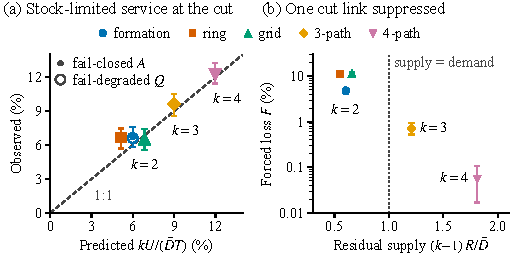
\includegraphics[width=\columnwidth]{fig2_cut_scaling.pdf}
\caption{Scaling with cut size $k$ on five graphs (twelve seeds, 95\% intervals).
Ring and grid are offset sideways for legibility. (a) Under a held cut, fail-closed $A$ and fail-degraded $Q$ follow the stock-limited prediction $kU/(\bar DT)$ of~(\ref{eq:cut}), $U=1.03$\,Mbit per link. (b) With one cut link suppressed, forced loss stays small
unless the $k-1$ remaining links ($R=240$\,bit/s) cannot carry the demand $\bar D$.}
\label{fig:scale}
\end{figure}

\subsection{Key-aware routing under a fallback}\label{sec:routing}
\textbf{(1) Availability.} A post-quantum fallback succeeds wherever a classical path
exists, so unattacked key-aware and shortest-path routing give identical fail-degraded
availability in every seed and condition; the zero-width interval is an identity of
the model, not a measured precision. $Q$ still separates them: key-aware routing
raises it by 0.12 points (CI $[0.05,0.19]$) for 5.0\,Mbit (CI $[2.3,7.7]$) more key per
day.

\textbf{(2) Hop penalty.} At ISR factor 1, key-aware routing loses 2.6 points of
fail-closed service to shortest path (CI $[-2.9,-2.3]$), but only when measured after a
12\,h warm-up from full stores, by which time it has left less stock for ISR. Measured
from $t=0$ it gains 0.08 points, from 2\% fill 0.11--0.13, and at the rescaled load
0.13 (CI $[0.07,0.20]$), so the penalty is a warm-up transient. The hop multiplier costs key but little service; the 25--40\% gains reported
in~\cite{cvitic} measure blocking without a fallback.

\textbf{(3) Reservation floors.} Class-aware floors~\cite{mehic} reserving 20 and 40\%
of each store against ISR and LOG work as an admission decision rather than a graded
control. At 2\% fill they deny logistics its quantum key (fail-closed service
$-37.6$ points, logistics 98.9$\rightarrow$0\%), and fail-degraded operation then
forces 2.1\% below ITS with no adversary present; at full stock and the rescaled load
they have no effect. Under the cut, the denial buys endurance: $+14.3$ points of
fail-closed service (CI $[13.4,15.2]$) and $F$ down from 90.1 to 63.6\%, because
logistics' hybrid debits stop draining the cut.

\subsection{Downgrade-forcing cost versus depth}\label{sec:cost}
\begin{figure}[t]
\centering
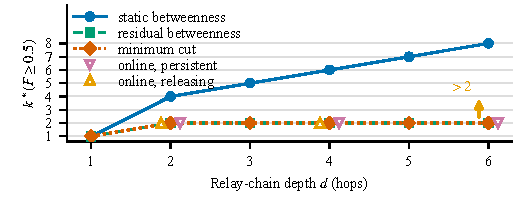
\includegraphics[width=\columnwidth]{fig3_forcing_cost.pdf}
\caption{Forcing cost $k^\ast$, the smallest budget whose mean forced loss reaches
50\% in 24\,h, against chain depth (fail-degraded, 2\% fill, eight seeds; online
adversaries: six seeds, at most two links; arrow: not reached).}
\label{fig:cost}
\end{figure}

For $d\ge2$ every link of the depth-$d$ chain lies on one cycle with equal
betweenness, so a static centrality ranking is decided by its tie order. Ours attacks
the longer alternate first and needs $d+2$ links to force half the entitled traffic
below ITS (another tie order needs $d+1$). Recomputing betweenness on the residual
graph after each removal needs only the minimum cut, two links, at every depth
$d\ge2$ (Fig.~\ref{fig:cost}). An online adversary that sees only committed routes and
updates every 60\,s holds a cut from its first choice if it keeps its slots
(89.7--92.9\% at depths 2, 4 and 6; 48 link-hours). If it releases slots while its
path is briefly unreachable, forced loss falls with depth from 72.3 to 35.5\%, as
longer paths are unreachable more often and released links refill. The linear growth
under a static ranking therefore overstates resilience; against residual betweenness
or a cut-holding adversary, depth buys no protection. Per-link costs do matter on the
formation: with the fibre 10 or 100 times dearer, residual betweenness avoids it and
forces 10.1\% at budget two instead of 89.8\%, and the fibre-free cut is unaffected.

\subsection{Sensitivity and operating envelope}\label{sec:sens}
\begin{table}[t]
\caption{Capability against budget: forced assurance loss $F$ (\%) after a 24\,h
attack from 2\% usable fill, outage-free, eight seeds; $\pm$ is the larger side of
the 95\% bootstrap interval. Complete suppression starts at $\Delta e=0.045$.}
\label{tab:envelope}
\centering\scriptsize
\setlength{\tabcolsep}{1.6pt}
\begin{tabular}{@{}lrrrrrrr@{}}
\toprule
 & & \multicolumn{4}{c}{$\gamma=1$, $\Delta e=$} & \multicolumn{2}{c}{$\gamma=3.4$, $\Delta e=$}\\
\cmidrule(lr){3-6}\cmidrule(l){7-8}
Graph & $b$ & 0.03 & 0.04 & 0.045 & 0.05 & 0.03 & 0.04\\
\midrule
Formation & 1 & 0 & $<$0.1 & 0 & 0 & 0.47$\pm$0.06 & 0.15$\pm$0.05\\
 & 2 & $<$0.1 & $<$0.1 & 93.1$\pm$0.9 & 93.1$\pm$0.9 & 63.0$\pm$1.0 & 88.8$\pm$0.9\\
 & 3 & $<$0.1 & $<$0.1 & 93.1$\pm$0.9 & 93.1$\pm$0.9 & 63.0$\pm$1.0 & 88.8$\pm$0.9\\
\addlinespace[1pt]
3-path & 2 & 0 & 0 & $<$0.1 & $<$0.1 & 0 & 0\\
 & 3 & 0 & 0 & 90.4$\pm$0.7 & 90.4$\pm$0.7 & 41.6$\pm$0.8 & 83.8$\pm$0.9\\
 & 4 & 0 & 0 & 90.4$\pm$0.7 & 90.4$\pm$0.7 & 41.6$\pm$0.8 & 83.8$\pm$0.9\\
\addlinespace[1pt]
4-path & 3 & 0 & 0 & $<$0.1 & $<$0.1 & 0 & $<$0.1\\
 & 4 & 0 & 0 & 87.7$\pm$1.1 & 87.7$\pm$1.1 & 17.3$\pm$0.9 & 78.2$\pm$1.7\\
 & 5 & 0 & 0 & 87.7$\pm$1.1 & 87.7$\pm$1.1 & 17.3$\pm$0.9 & 78.2$\pm$1.7\\
\bottomrule
\end{tabular}

\end{table}

\textbf{Capability.} A link at nominal $e_0$ aborts once $\Delta e\ge
e_{\mathrm{abort}}-e_0=0.045$. Below that it keeps $\rho(e)$ of its rate, and loss is
forced once the cut's residual supply nears the entitled classes' cheapest ITS demand,
about 72\,bit/s, plus the hybrid debits competing for it. The response shape
therefore matters below the threshold but not above it (Table~\ref{tab:envelope}). At
$\gamma=1$, sub-threshold injection forces under 0.1\% on the formation at any budget
up to five links; without outages and one link short of the cut, even
supra-threshold injection forces under 0.1\% (4.8\% with them, Table~\ref{tab:head});
and every budget from the cut upward gives the same 93.1\%. The larger cuts repeat the pattern. At $\gamma=3.4$ the attack bites earlier: $\Delta
e=0.03$ leaves 9.8\% of the rate and forces 63.0, 41.6 and 17.3\% at the three cuts
without aborting a link. Raising $e_{\mathrm{abort}}$ to 0.11 moves the threshold to
$\Delta e=0.068$ rather than the 0.08 that $e_{\mathrm{abort}}-e_0$ suggests, because
the ITS zero of~(\ref{eq:rho}), at 9.8\%, is reached first; $\Delta e=0.06$ already
forces 40.9\% on the three-link cut.

\textbf{Endurance.} Sensitivity runs use eight seeds (headline cell $F=89.9\%$,
fail-closed $A=7.0\%$). Initial fills of 2, 10 and 100\% give $F=89.9$, 65.4 and 0\%,
and 1, 6 and 24\,h attacks at 2\% fill give 0.06, 17.6 and 89.9\%, with first forcing
after about 1.5\,h, the $T^\ast$ of~(\ref{eq:cut}). The same bound predicts 7.2 and
72\,h at 10 and 100\% fill; we see a median first forcing of 6.6\,h and none within
24\,h. Stock matters from full stores as well. At ISR factor 1 and
$n_{\mathrm{auth}}=2$, after a 12\,h warm-up and under the two-link betweenness attack,
treating an aborted link's stock as unusable leaves 30.4\% fail-closed service and
$F=65.1\%$; spending it gives 76.7\% (paired $+46.4$ points, CI $[45.8,46.9]$) and
4.1\%. Forcing thus needs a per-link capability, a cost-weighted cut and an attack that outlasts the stock behind it.

\textbf{Load.} Unattacked, the fail-mode gap vanishes at sustainable load (paired
$\Delta A=0.00$ and $+0.01$ points at ISR factors 0.03 and 0.1) and appears only under
overload ($+17.2$ at factor 1). Under the cut it persists at every load ($\Delta
A=85.4$, 90.6 and 94.7 points), narrowing only because a lighter load drains the stock
more slowly, and $\Delta Q\le0$ holds throughout on the formation, so the ordering
never reverses.

\textbf{Authentication.} With $n_{\mathrm{auth}}$ of 2 or 40 instead of 7, fail-closed
service under the cut is 8.5 or 3.3\% (7.0\%) and $F$ 87.9 or 93.5\% (89.9\%). At 40
the unattacked formation already forces 3.7\%, so policy differences do not simply cancel.

\textbf{Correlated weather.} Weather alone can sever the cut. Up/down times of
900/600\,s give an unattacked $F$ of 1.7\% (independent links) and 3.0\% (all
free-space generation failing together) and lower unattacked fail-closed service to
95.4 and 94.2\%, while the paired attack excess stays at 88.1 and 86.9 points. Since
$F$ counts loss whatever its cause, attribution needs the weather-matched baseline; a
held correlated outage looks like an attack of the same duration.

\textbf{Classical channel.} Fail-degraded availability survives QBER attack only
because aborted links keep their classical channels; denying transport on the cut
drops both modes to 0.06\%. Pre-placed symmetric keys cannot change this, since
ciphertext still needs a path, but they do remove the dependence on a live
key-establishment service. With that service down under the held cut, an online KEM
fallback serves 5.0\% and pre-placed keys 97.5\%, still forcing 89.9\% below ITS.
Pre-placed keys thus move the dependency without reducing the assurance loss. Their
lifetime, refresh and distribution cost are not modelled, so their 97.5\% is an upper
bound.

\subsection{Policy-space audit with a learned controller}\label{sec:audit}
\begin{table}[t]
\caption{Learned grade controllers against the budget-greedy heuristic on the frozen
test set (seven conditions, twelve held-out seeds): paired differences, 95\%
intervals; $J$ in $10^{-3}$, others in points. $^\ast$Never below the floor; also the 24\,h nominal result.}
\label{tab:learn}
\centering\footnotesize
\setlength{\tabcolsep}{1.2pt}
\begin{tabular}{@{}lccc@{}}
\toprule
 & Strict floor$^\ast$ & 6\,h nominal & Multi-condition\\
\midrule
$\Delta J$ ($10^{-3}$) & $-3.6$ {\tiny$[-4.0,-3.4]$} & $-4.7$ {\tiny$[-5.8,-3.5]$} & $+1.1$ {\tiny$[+0.2,+2.0]$}\\
$\Delta Q$ & $+0.04$ {\tiny$[0.00,+0.06]$} & $-0.08$ {\tiny$[-0.19,+0.04]$} & $+0.10$ {\tiny$[+0.01,+0.20]$}\\
$\Delta Q_{\mathrm{ISR}}$ & $+0.25$ {\tiny$[+0.14,+0.36]$} & $-0.21$ {\tiny$[-0.36,-0.05]$} & $-2.77$ {\tiny$[-2.97,-2.59]$}\\
$\Delta F_B$ & $-1.99$ {\tiny$[-2.03,-1.94]$} & $-1.99$ {\tiny$[-2.03,-1.94]$} & $+1.71$ {\tiny$[+1.55,+1.85]$}\\
\bottomrule
\end{tabular}

\end{table}

A better score in our own simulator would prove little, so we ask how much room a
budget-greedy heuristic (the strongest affordable grade within the shield) leaves. The
cross-entropy method~\cite{cem} searches an 18-state, five-action grade table for
$J=A-0.75L$ behind a per-class shield~\cite{shield} that caps class-$c$ violations at
$\lfloor\epsilon_cN_c(t)\rfloor$, with $\epsilon=(0,0.1,0.1)$ for (C2, ISR, LOG). Six
training, four validation and twelve test seeds are disjoint, and tables were frozen
before testing on seven conditions, two on unseen graphs (Table~\ref{tab:learn}).

Trained on nominal, attacked and severe-weather runs, the learner gains $\Delta
J=+1.1\times10^{-3}$; that the heuristic reaches 99.8\% of this reflects our search
budget more than the room left. The gain spends ISR's allowance where it costs the
most one-time-pad payload (ISR $Q$ $-2.8$ points, $F_B$ $+1.7$), under every class
weighting. As $\Delta J$ is linear in the weights, reversal prices follow by algebra
once the search supplies a candidate: the heuristic beats the strict floor for
$\lambda<0.98$ (CI $[0.96,1.00]$) in $J=A-\lambda L$, while the learned gain is
insensitive to $\lambda$ and reverses at a forced-loss price $\mu^\ast=0.32$ (CI
$[0.06,0.60]$; $\Delta F=+0.33$ points). Tables trained on nominal traffic alone lose
on all the stressed conditions, because nominal runs never reach depletion, a failure
the training curves do not show. The per-class shield is also spent where scoring is
cheapest, so floors must be specified \emph{and} priced per class.

\section{Discussion and Limitations}
Choosing between refusal and degradation amounts to choosing whether the adversary
takes availability or assurance. For operators, three rules follow: report
$Q$ and $F$ beside $A$; provision stock behind the minimum cut for $T^\ast$ hours of
the attacks of concern; and set fail modes and exception allowances per class, pricing
each allowance. The study has limitations. Key rates are parameterised (no photonics is simulated), response shapes are illustrative, relays are trusted and detector
blinding is invisible by construction. Weights are exposure proxies, and fill, outages
and attack costs are declared scenarios, which we sweep. No cipher or
KEM is executed, the policy search was modest and the five graphs are synthetic. Next
steps are QKDNetSim cross-validation and a reimplemented published router. Y.3803 asks
key managers to record the relay method and prefer OTP-relayed keys for QKD-level
requests~\cite{itu3803}, but the ETSI interface~\cite{etsi014} still exposes no grade
a consumer could enforce.

\section{Conclusion}
Standards permit fallback to weaker key supply, while a layered post-quantum design
forbids it as a downgrade attack. Holding the formation's minimum cut for a day either
collapses fail-closed service from 97.5\% to 6.7\% or keeps 97.5\% served while only
6.6\% meets its authorised grade and 90.1\% of entitled traffic is forced below ITS
protection; on all five graphs a held cut forces 87.6--92.9\%. Forcing takes a per-link
capability, a cost-weighted cut and an attack that outlasts the stock behind the cut.
A fallback also needs the classical channel, and a learned controller pays for its
small gain with one-time-pad payload. We argue that QKD resilience reporting should
cover the assurance-grade composition of \emph{served} traffic alongside key-supply
continuity.

\section*{Reproducibility and Acknowledgements}
A large language model assisted with coding and drafting; all modelling decisions,
parameter provenance, experimental design and claims are the authors', and every
reported number comes from the released simulator, configurations, per-seed results,
validation gate and figure and table scripts at
\url{https://github.com/LakshyaJ1/Quantum_ResearchPaper}.

\begin{thebibliography}{00}
\bibitem{salvail} L. Salvail \emph{et al.}, ``Security of trusted repeater quantum key distribution networks,'' \emph{J. Comput. Secur.}, vol.~18, no.~1, pp.~61--87, 2010.
\bibitem{itu3803} \emph{Quantum Key Distribution Networks---Key Management}, ITU-T Rec.~Y.3803, Dec. 2020, cl.~8.2.3--8.2.5.
\bibitem{makris} N. Makris \emph{et al.}, ``Field demonstration of a fully managed, L1 encrypted 3-node network with hybrid relayed-QKD and centralized symmetric classical key management,'' in \emph{Proc. ECOC}, 2024.
\bibitem{tysowski} P.~K. Tysowski, X. Ling, N. L\"utkenhaus, and M. Mosca, ``The engineering of a scalable multi-site communications system utilizing quantum key distribution (QKD),'' \emph{Quantum Sci. Technol.}, vol.~3, no.~2, 024001, 2018.
\bibitem{spooren} P. Spooren, A. Neuhold, S. Ramacher, and T. H\"uhn, ``PQC-enhanced QKD networks: A layered approach,'' in \emph{Proc. IEEE QCNC}, Kobe, Japan, 2026, pp.~354--358, doi:10.1109/QCNC69040.2026.00060.
\bibitem{schartner} P. Schartner and S. Rass, ``Quantum key distribution and denial-of-service: Using strengthened classical cryptography as a fallback option,'' in \emph{Proc. Int. Comput. Symp.}, 2010, pp.~131--136.
\bibitem{vanduijn} T. van Duijn, S.~R. Verschoor, S. Rommel, and I. Tafur Monroy, ``Routing strategies for quantum key distribution networks based on trusted relay nodes,'' in \emph{Proc. ONDM}, 2024.
\bibitem{johann} T. Johann \emph{et al.}, ``Comparison and optimization of different routing methods for meshed QKD networks using trusted nodes,'' \emph{J. Opt. Commun. Netw.}, vol.~16, no.~3, pp.~382--391, 2024.
\bibitem{hao} Y. Hao, Y. Xie, W. Gao, and J. Tang, ``Q-learning for resource-aware and adaptive routing in trusted-relay QKD network,'' \emph{Photonics}, vol.~12, no.~10, 969, 2025.
\bibitem{mehic} M. Mehic \emph{et al.}, ``A novel approach to quality-of-service provisioning in trusted relay quantum key distribution networks,'' \emph{IEEE/ACM Trans. Netw.}, vol.~28, no.~1, pp.~168--181, 2020.
\bibitem{cao} Y. Cao, Y. Zhao, C. Colman-Meixner, X. Yu, and J. Zhang, ``Key on demand (KoD) for software-defined optical networks secured by quantum key distribution (QKD),'' \emph{Opt. Express}, vol.~25, no.~22, pp.~26453--26467, 2017.
\bibitem{sanz} A. Sanz \emph{et al.}, ``QuLore: An adaptive security framework to extend quantum-safe communications to real-world networks,'' arXiv:2511.22416v2, 2026.
\bibitem{zhu} Z. Zhu, ``Techno-economic feasibility analysis of quantum key distribution for power-system communications,'' arXiv:2510.15248, 2025.
\bibitem{li} M. Li \emph{et al.}, ``Routing and wavelength assignment with minimal attack radius for QKD networks,'' in \emph{Proc. IEEE GLOBECOM}, 2025, pp.~4071--4076.
\bibitem{ghorab} E.~M. Ghourab, M. Azab, and D. Gra\v{c}anin, ``A quantum key distribution routing scheme for a zero-trust QKD network system: A moving target defense approach,'' \emph{Big Data Cogn. Comput.}, vol.~9, no.~4, 76, 2025.
\bibitem{hafeez} S. Hafeez \emph{et al.}, ``Quantum-secured routing in drone communication for 6G-enabled smart mobility,'' \emph{Sci. Rep.}, vol.~16, 8626, 2026.
\bibitem{cvitic} I. Cviti\'c, D. Perakovi\'c, and A.~N. Pinto, ``Overview of routing approaches in quantum key distribution networks,'' in \emph{Proc. FABULOUS 2025}, LNICST, vol.~700, Springer, 2026, pp.~50--67.
\bibitem{agalya} A. Agalya and K. Priyadarsini, ``Trust-aware hybrid QKD--PQC key management for quantum-safe communication networks,'' \emph{Front. Commun. Netw.}, vol.~7, 1929455, 2026.
\bibitem{hernandez} J.~C. Hernandez-Hernandez \emph{et al.}, ``Sentinel-based failover for QKD-augmented IPsec tunnels,'' to appear in \emph{Proc. NetQSA, IEEE ICNP}, Oct. 2026, arXiv:2609.01121.
\bibitem{mehicdos} M. Mehic, S. Rass, E. Dervisevic, and M. Voznak, ``Tackling denial of service attacks on key management in software-defined quantum key distribution networks,'' \emph{IEEE Access}, vol.~10, pp.~110512--110520, 2022.
\bibitem{ietfhybrid} D. Stebila, S. Fluhrer, and S. Gueron, ``Hybrid key exchange in TLS 1.3,'' IETF RFC 9954, Jul. 2026, \S1.1.
\bibitem{qkdnetsim} M. Mehic, O. Maurhart, S. Rass, and M. Voznak, ``Implementation of quantum key distribution network simulation module in the network simulator NS-3,'' \emph{Quantum Inf. Process.}, vol.~16, no.~10, 253, 2017.
\bibitem{peev} M. Peev \emph{et al.}, ``The SECOQC quantum key distribution network in Vienna,'' \emph{New J. Phys.}, vol.~11, 075001, 2009.
\bibitem{etsi014} \emph{Quantum Key Distribution (QKD); Protocol and Data Format of REST-Based Key Delivery API}, ETSI GS QKD 014 V1.1.1, Feb. 2019.
\bibitem{alleaume} R. All\'eaume \emph{et al.}, ``Using quantum key distribution for cryptographic purposes: A survey,'' \emph{Theor. Comput. Sci.}, vol.~560, pp.~62--81, 2014.
\bibitem{sasaki} M. Sasaki \emph{et al.}, ``Field test of quantum key distribution in the Tokyo QKD Network,'' \emph{Opt. Express}, vol.~19, no.~11, pp.~10387--10409, 2011.
\bibitem{lydersen} L. Lydersen \emph{et al.}, ``Hacking commercial quantum cryptography systems by tailored bright illumination,'' \emph{Nat. Photonics}, vol.~4, no.~10, pp.~686--689, 2010.
\bibitem{walenta} N. Walenta \emph{et al.}, ``A fast and versatile quantum key distribution system with hardware key distillation and wavelength multiplexing,'' \emph{New J. Phys.}, vol.~16, 013047, 2014.
\bibitem{fung} C.-H.~F. Fung, X. Ma, and H.~F. Chau, ``Practical issues in quantum-key-distribution postprocessing,'' \emph{Phys. Rev. A}, vol.~81, 012318, 2010.
\bibitem{stucki} D. Stucki \emph{et al.}, ``Long-term performance of the SwissQuantum quantum key distribution network in a field environment,'' \emph{New J. Phys.}, vol.~13, 123001, 2011.
\bibitem{chen} T.-Y. Chen \emph{et al.}, ``Implementation of a 46-node quantum metropolitan area network,'' \emph{npj Quantum Inf.}, vol.~7, 134, 2021.
\bibitem{dynes} J.~F. Dynes \emph{et al.}, ``Cambridge quantum network,'' \emph{npj Quantum Inf.}, vol.~5, 101, 2019.
\bibitem{cem} R. Rubinstein, ``The cross-entropy method for combinatorial and continuous optimization,'' \emph{Methodol. Comput. Appl. Probab.}, vol.~1, no.~2, pp.~127--190, 1999.
\bibitem{shield} M. Alshiekh \emph{et al.}, ``Safe reinforcement learning via shielding,'' in \emph{Proc. AAAI}, 2018, pp.~2669--2678.
\end{thebibliography}
\end{document}
